\begin{figure}[H]
    \centering

    \caption{A timeseries of the energy consumption over time for DUT 2 when running PCM for all cores}
    \label{fig:exp_3_dut_2_pcm_timeseries_all_cores}
\end{figure}

\begin{tikzpicture}
    \pgfplotsset{
        width=1.0\textwidth,
        height=0.25\textheight
    }
    \begin{axis}[
        % title={Temperature dependence of CuSO\(_4\cdot\)5H\(_2\)O solubility},
        xlabel={Time (s)},
        ylabel={Energy Consumption (w)},
        xmin=0, xmax=700,
        ymin=0, ymax=60,
        % xtick={0,20,40,60,80,100},
        % ytick={0,20,40,60,80,100,120},
        legend pos=north west,
        ymajorgrids=true,
        grid style=dashed,
    ]
    
    \addplot[
        color=blue,
        % mark=square,
        ]
        coordinates {

        };
        % \legend{CuSO\(_4\cdot\)5H\(_2\)O}
        
    \end{axis}
    \end{tikzpicture}